\documentclass{article}
\usepackage[margin=0.5in]{geometry}
\usepackage{tikz}
\usepackage{graphicx}
\usepackage{listings}
\usepackage{amsmath}
\usepackage{xcolor}
\usepackage{hyperref}
\hypersetup{
    colorlinks=true,
    linkcolor=blue,
    filecolor=magenta,      
    urlcolor=cyan,
    pdftitle={Overleaf Example},
    pdfpagemode=FullScreen,
}

\definecolor{bashkeyword}{RGB}{0,0,255}
\definecolor{bashstring}{RGB}{42,0,255}
\definecolor{bashcomment}{RGB}{0,128,0}

\lstdefinestyle{bashstyle}{
    language=bash,
    basicstyle=\ttfamily,
    keywordstyle=\color{bashkeyword},
    stringstyle=\color{bashstring},
    commentstyle=\color{bashcomment},
    numbers=left,
    numberstyle=\small\color{gray},
    stepnumber=1,
    numbersep=8pt,
    backgroundcolor=\color{white},
    showspaces=false,
    showstringspaces=false,
    frame=single,
    rulecolor=\color{black},
    tabsize=2,
    captionpos=b,
    breaklines=true,
    breakatwhitespace=true,
    escapeinside={(*@}{@*)},
    xleftmargin=4pt,
    framexleftmargin=5pt,
    framexrightmargin=5pt,
}

\title{SPIDR Analysis Documentation}
\author{Darvesh Gorhe}

\begin{document}
    \maketitle
    \tableofcontents

    \section{Introduction}
    This document outlines the SPIDR analysis pipeline, which has three main sections: preprocessing, postprocessing, and downstream analysis. Each section covers the following:
    
    \begin{align*}
        \text{Preprocessing:} & & \text{fastq} \rightarrow \text{bed} \\
        \text{Postprocessing:} & & \text{bed} \rightarrow \text{bedgraph, bigwig} \\
        \text{Downstream Analysis:} & & \text{bedgraph, bigwig} \rightarrow \text{tables, figures, etc.} \\
    \end{align*}

    \noindent Preprocessing and Postprocessing use Snakemake to orchestrate several steps in an efficient way. Snakemake allows each pipeline to effectively use high-performance computing resources with minimal human supervision. This implementation allows Snakemake to either submit batch jobs or run interactively.
    \vspace{5mm}
    
    \noindent In many cases, it is \textit{impossible} to run the pipeline on a local machine due to the large amount of data, computational requirements, and unavailable dependencies. With respect to the dependencies, this is particularly an issue for things like \texttt{samtools}, \texttt{deeptools}, and \texttt{pysam}. These tools are often only designed and supported for Linux machines.
    \pagebreak

    \section{Setting Up your HPC Cluster Environment}
    The following steps are not strictly necessary, but they will make your life much easier. The steps below show you how to install \texttt{mamba} outside of your home directory. This is necessary because Snakemake uses the mamba dependency resolver by default and your home directory is somewhat limited in space and permissions. For more detailed steps see the steps below, otherwise continue to the next section 3.
    \vspace{5mm}

    \noindent To explicitly use \texttt{conda} instead of \texttt{mamba}, you can add the following line to your \texttt{sbatch-run.sh} and \texttt{interactive-run.sh}: \texttt{--use-conda}.
    
    \subsection{Why should I do this?}
    \begin{itemize}
        \item Snakemake is very persistent in getting you to use \texttt{mamba}
        \item Sometimes \texttt{conda} does not work or takes an \textit{extremely} long time to resolve dependencies, especially for larger environment definition files (e.g. \texttt{pipeline/envs/sprite.yaml})
        \item \texttt{mamba} can also help down the line for testing and debugging \texttt{conda}/\texttt{mamba} environments.
    \end{itemize}

    \subsection{Steps}
    \begin{enumerate}
        \item Download Mambaforge from \href{https://github.com/conda-forge/miniforge#install}{this page}.
        
        \item Run the installation script from the same place you downloaded it. The command should be something like this, but defer to the instructions on the page you downloaded it from:
        \begin{lstlisting}[style=bashstyle]
            bash Mambaforge-$(uname)-$(uname -m).sh
        \end{lstlisting}
        
        \item Follow the prompts on screen. Stop when you get to the part where it asks you where to install mamba. For Ginsburg users, I'd recommend \texttt{/burg/mjlab/users/<your UNI>/cli-tools}. For other HPC users, determine what a good place is for you based on your permissions and space available.
        \begin{itemize}
            \item You may need to create the \texttt{<your UNI>} directory within \texttt{users} if it does not already exist. You can do so by running:
            \begin{lstlisting}[style=bashstyle]
                mkdir -p /burg/mjlab/projects/cli-tools/<your UNI>
            \end{lstlisting}
            \item Don't include the \texttt{<>} when you run the command. For example, my UNI is \texttt{dsg2157} so I would run:
            \begin{lstlisting}[style=bashstyle]
                mkdir -p /burg/mjlab/projects/cli-tools/dsg2157
            \end{lstlisting}
        \end{itemize}
        
        \item Within the instructions it will ask you if you want to run \texttt{conda init}. Type 'yes' (without the single quotes) and hit enter/return.

        \item To see the effects of the changes, you can either log out and log back into your cluster or you can run \texttt{source $\sim$/.bashrc} to reload your bash profile (which has the same effect).
        \begin{itemize}
            \item To check that \texttt{mamba} was installed correctly, run:
            \begin{lstlisting}[style=bashstyle]
                mamba --version
            \end{lstlisting}

            \item The output should look something like this (your version numbers may be different):
            \begin{lstlisting}[style=bashstyle]
                mamba 1.4.1
                conda 23.1.0
            \end{lstlisting}
        \end{itemize}
    \end{enumerate}
    \pagebreak
    \section{Preprocessing}
    \subsection{How to Run \texttt{generate-targets.smk}}
    \begin{enumerate}
        \item Navigate to the \texttt{spidr} repository on your machine (i.e. Ginsburg or your institution's HPC).
        
        \item Create a directory within the \texttt{pipeline} directory called \texttt{fastq\_files}.
        \begin{lstlisting}[style=bashstyle]
            mkdir -p fastq_files
        \end{lstlisting}
        
        \item Copy or move your read 1 and read 2 fastq files into the \texttt{fastq\_files} directory you just created. Make sure that the fastq files are compressed using \texttt{gzip}.
        \begin{itemize}
            \item For larger files, consider using \texttt{pigz} which allows for parallel compression with multiple threads (\texttt{-p -1} tells \texttt{pigz} to use all available threads)
            \begin{lstlisting}[style=bashstyle]
                pigz -p -1 <read_1 file>.fastq
                pigz -p -1 <read_2 file>.fastq
            \end{lstlisting}
            \item Compressing your \texttt{fastq} files is important because many steps in the Snakemake pipeline assume that the fastq files are compressed. As a result, these steps use programs designed to work specifically with compressed files (e.g. \texttt{zcat})
            \item Make sure your files are in the following format:
            \begin{lstlisting}[style=bashstyle]
                <experiment>_R[1|2].fastq.gz
            \end{lstlisting}
            \item In this case \texttt{[1|2]} means either \texttt{1} or \texttt{2}. For example, if your experiment is called \texttt{my\_experiment} then your files should be named:
            \begin{lstlisting}[style=bashstyle]
                my_experiment_R1.fastq.gz
                my_experiment_R2.fastq.gz
            \end{lstlisting}
        \end{itemize}
        
        \item Run \texttt{python fastq2json.py -f fastq\_files} from the \texttt{pipeline} directory. This will create a \texttt{samples.json} file which will be used by the pipeline to determine which fastq files to run.
        \begin{lstlisting}[style=bashstyle]
            python fastq2json.py -f fastq_files
        \end{lstlisting}

        \item Modify the \texttt{cluster.generate-targets.yaml} file to reflect your account ID. You can change other parameters as well, but the \texttt{account} parameter is the only one you need to change. The account parameter should be the one that you use to submit jobs to the cluster (\texttt{mjlab} for anyone in the lab using Ginsburg). To show this more concretely, here's a snippet of the \texttt{cluster.generate-targets.yaml} file:
        \begin{lstlisting}[style=bashstyle]
            __default__:
                account: "mjlab" # <-- Change this to your account ID
                time: "01:00:00"
                mem: 20g 
                cpus: 1
                nodes: 1
                output: "workup/logs/cluster/{rule}.{wildcards.sample}.out"
                error: "workup/logs/cluster/{rule}.{wildcards.sample}.err"
            splitfq:
                account: "mjlab" # <-- Change this to your account ID
                time: "02:00:00"
                mem: 64g 
                cpus: 1
                nodes: 1
                output: "workup/logs/cluster/{rule}.{wildcards.sample}.out"
                error: "workup/logs/cluster/{rule}.{wildcards.sample}.err"
            compress_fastq:
                account: "mjlab" # <-- Change this to your account ID
                time: "02:00:00"
                mem: 64g 
                cpus: 8
                nodes: 1
                output: "workup/logs/cluster/{rule}.{wildcards.sample}.out"
                error: "workup/logs/cluster/{rule}.{wildcards.sample}.err"
            ...
        \end{lstlisting}

        \item Modify \texttt{config.generate-targets.yaml} to your liking. This config file looks like this
        
        \begin{lstlisting}[style=bashstyle]
            # email to which errors will be sent
            email: "dsg2157@columbia.edu"
            
            # Location of the config file for barcodeIdentification
            bID: "config_6_rounds_mTOR.txt"
            
            # Location of the samples json file produced with the fastq2json.py script 
            samples: "./samples.json"
            
            # Output directory  
            output_dir: ""
            
            # Temporary directory
            temp_dir: "/burg/mjlab/projects/spidr_preprocessing_dg/scratch"
            
            # Unique tags in the ROUND1 tags within config
            conditions: ['CNTRL', 'TORIN']
            
            # Currently "mm10" and "hg38" available
            assembly: "hg38"
            
            proportion: 0.7
            
            min_oligos: 3
            
            # Number of barcodes used
            num_tags: "7"
            
            # Number of chunks to split fastq
            num_chunks: 10
            
            # Format for splitting clusters
            rounds_format: 'format_6_rounds_mTOR.txt'
            
            # File for cutadapt
            cutadapt_oligos: "oligo2_reverse.fasta"
            
            # Bowtie2 Indexes
            # Note: mm10 index currently not available at specified filepath
            bowtie2_index:
                hg38: "/burg/mjlab/projects/spidr_preprocessing_dg/ncRNA_bt2/ncRNA"
            
            # Star Indexes
            # Note: mm10 index currently not available at specified filepath
            star_index:
                hg38: "/burg/mjlab/projects/spidr_preprocessing_dg/hg38"
        \end{lstlisting}

        \begin{itemize}
            \item The most likely things that you need to change are: \texttt{conditions}, \texttt{assembly}, \texttt{bowtie2\_index}, \texttt{star\_index}, \texttt{bID}, \texttt{rounds\_format}, and \texttt{num\_tags}.
            \item You may need to change \texttt{cutadapt\_oligos} if you've used modified adapater sequences.
            \item You may want to change \texttt{num\_chunks} if you have large fastq files. Generally, higher is better if your cluster has the capacity to process many jobs in parallel. Otherwise, lower is fine. 10 is a good number to start with.
            \item Everything else you can experiment with.
            \item It should be noted that \texttt{output\_dir} is not well supported so it's recommended to leave it as an empty string (i.e. what's shown in the example above).
        \end{itemize}

        \item Check that Snakemake is installed by running the following (you should get an output like \texttt{7.25.0})
        \begin{lstlisting}[style=bashstyle]
            snakemake --version
        \end{lstlisting}
        \begin{itemize}
            \item If it's not installed then you can install it with \texttt{mamba} (or \texttt{conda}) in your current environment with:
            \begin{lstlisting}[style=bashstyle]
                mamba install -c conda-forge snakemake
            \end{lstlisting}

            \item It's recommended that you install Snakemake in your base environment for convenience. This specifically helps with \texttt{sbatch} jobs since loading anaconda on SLURM systems usually defaults to loading the base environment.
        \end{itemize}

        \item For interactive runs, run the following command (otherwise skip to the next step):
        \begin{lstlisting}[style=bashstyle]
            bash interactive-run.sh generate
        \end{lstlisting}

        \item For \texttt{sbatch} runs, run the following command:
        \begin{lstlisting}[style=bashstyle]
            bash sbatch-run.sh generate
        \end{lstlisting}
        \begin{itemize}
            \item You can check the status of the jobs that Snakemake dispatches by running:
            \begin{lstlisting}[style=bashstyle]
                squeue -u <your UNI>
            \end{lstlisting}
            
            \item when you submit the \texttt{sbatch} job you'll get a job id and hopefully a corresponding output file in the format: \texttt{slurm-<job id>.out}. You enter that file and you will see the outputs of the snakemake pipeline (similar to what you would see in your terminal if you ran the pipeline interactively).
        \end{itemize}
    \end{enumerate}
    
    \subsection{Relationship Between Files}
    \noindent Below is a schematic of how various files in the pipeline are related to one another. The file at the head of the arrow uses data provided by the file at the tail of the arrow. For example, \texttt{interactive-run.sh} is using information from \texttt{cluster.generate-targets.yaml}. As you can see, both are the same in terms of their relationship to one another. The only difference is how it's run.

    \begin{itemize}
        \item \texttt{interactive-run.sh} allows you to see the progress of the pipeline as it runs.
        \item \texttt{sbatch-run.sh} submits the pipeline to the cluster as a batch job.
        \item You can check the status of the pipeline on any SLURM system with \texttt{squeue -u <your UNI>}
    \end{itemize}

    \begin{figure}[ht]
        \centering
        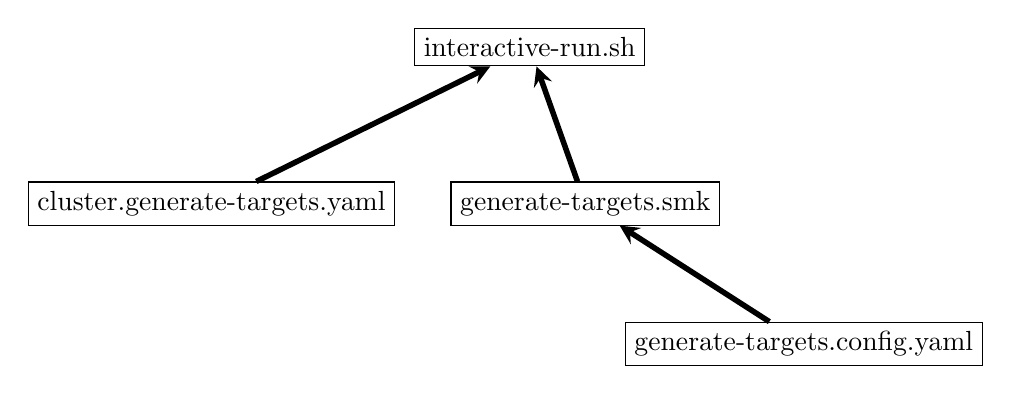
\begin{tikzpicture}
            % Nodes
            \node[draw] (run_pipeline) {interactive-run.sh};
            \node[draw, below left of=run_pipeline, align=center, below left=1cm] (cluster_yaml) {cluster.generate-targets.yaml};
            \node[draw, below right of=run_pipeline, align=center, below=1cm] (Snakefile) {generate-targets.smk};
            \node[draw, below of=Snakefile, align=center, below right=0.5cm] (config_yaml) {generate-targets.config.yaml};
            
            % Arrows
            \draw[->, >=stealth, line width=2pt] (cluster_yaml) -- (run_pipeline);
            \draw[->, >=stealth, line width=2pt] (Snakefile) -- (run_pipeline);
            \draw[->, >=stealth, line width=2pt] (config_yaml) -- (Snakefile);
        \end{tikzpicture}
        \caption[short]{Overview of preprocessing configuration with the interactive pipeline.}
    \end{figure}
    \begin{figure}[ht]
        \centering
        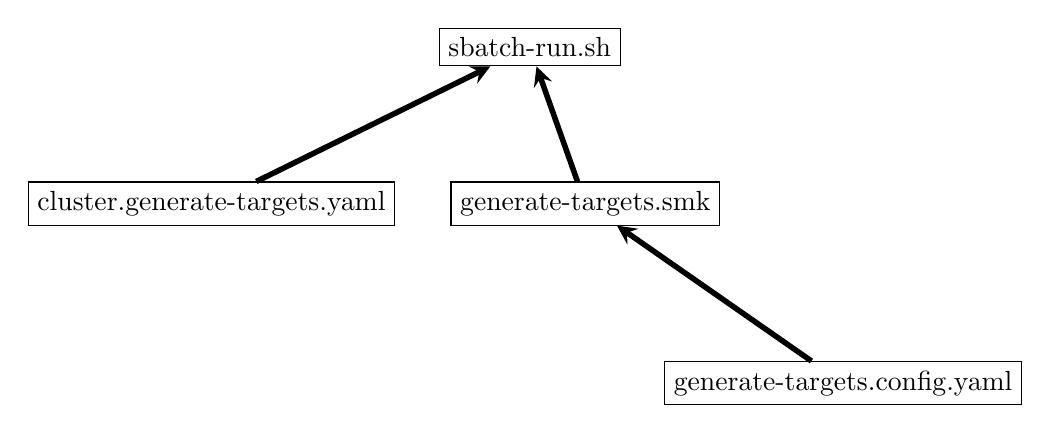
\begin{tikzpicture}
            % Nodes
            \node[draw] (run_pipeline) {sbatch-run.sh};
            \node[draw, below left of=run_pipeline, align=center, below left=1cm] (cluster_yaml) {cluster.generate-targets.yaml};
            \node[draw, below right of=run_pipeline, align=center, below=1cm] (Snakefile) {generate-targets.smk};
            \node[draw, below of=Snakefile, align=center, below right=1cm] (config_yaml) {generate-targets.config.yaml};
            
            % Arrows
            \draw[->, >=stealth, line width=2pt] (cluster_yaml) -- (run_pipeline);
            \draw[->, >=stealth, line width=2pt] (Snakefile) -- (run_pipeline);
            \draw[->, >=stealth, line width=2pt] (config_yaml) -- (Snakefile);
        \end{tikzpicture}
        \caption[short]{Overview of preprocessing configuration with the sbatch pipeline.}
    \end{figure}

    \subsection{Details of \texttt{generate-targets.smk}}

    \noindent Rules are chained together automatically based on the name of input and output file specified within each rule. Snakemake will create a directed acyclic graph (DAG) upon launching the pipeline. A DAG is a data structure which tells Snakemake the dependencies between rules. This allows Snakemake to determine in what order to execute the rules. Snakemake will then run the rules in the correct order and in parallel when possible. Below is an example of a DAG for the preprocessing pipeline with \texttt{num\_chunks}$=2$. As the number of chunks becomes larger, the middle of the graph becomes correspondingly wider.

    \begin{center}
        \includegraphics[scale=0.5]{../../pipeline/rulegraph-generate-targets.pdf}
    \end{center}

    \noindent Each node corresponds to a different rule. To see the contents of each rule you can view the \texttt{generate-targets.smk} file. The arrows represent the flow of data and the dependencies between rules. A rule will not run until all of its dependencies have successfully completed.

    \section{Postprocessing Pipeline}
    I'm not sure how the post-processing pipeline works to be completely honest, so I'm not comfortable writing documentation for it.

    \section{Downstream Analysis (Ahmed)}
    Not sure where Ahmed's code and figures are located.

    \section{Downstream Analysis (Darvesh)}
    Below is a comparison of the ENCODE data to the outputs of SPIDR. Specifically, we compare the transcript proportion as given by the supplementary data of ENCODE along with the ENCODE raw data processed through the same pipeline as the SPIDR data.
    \begin{figure}[ht]
        \centering
        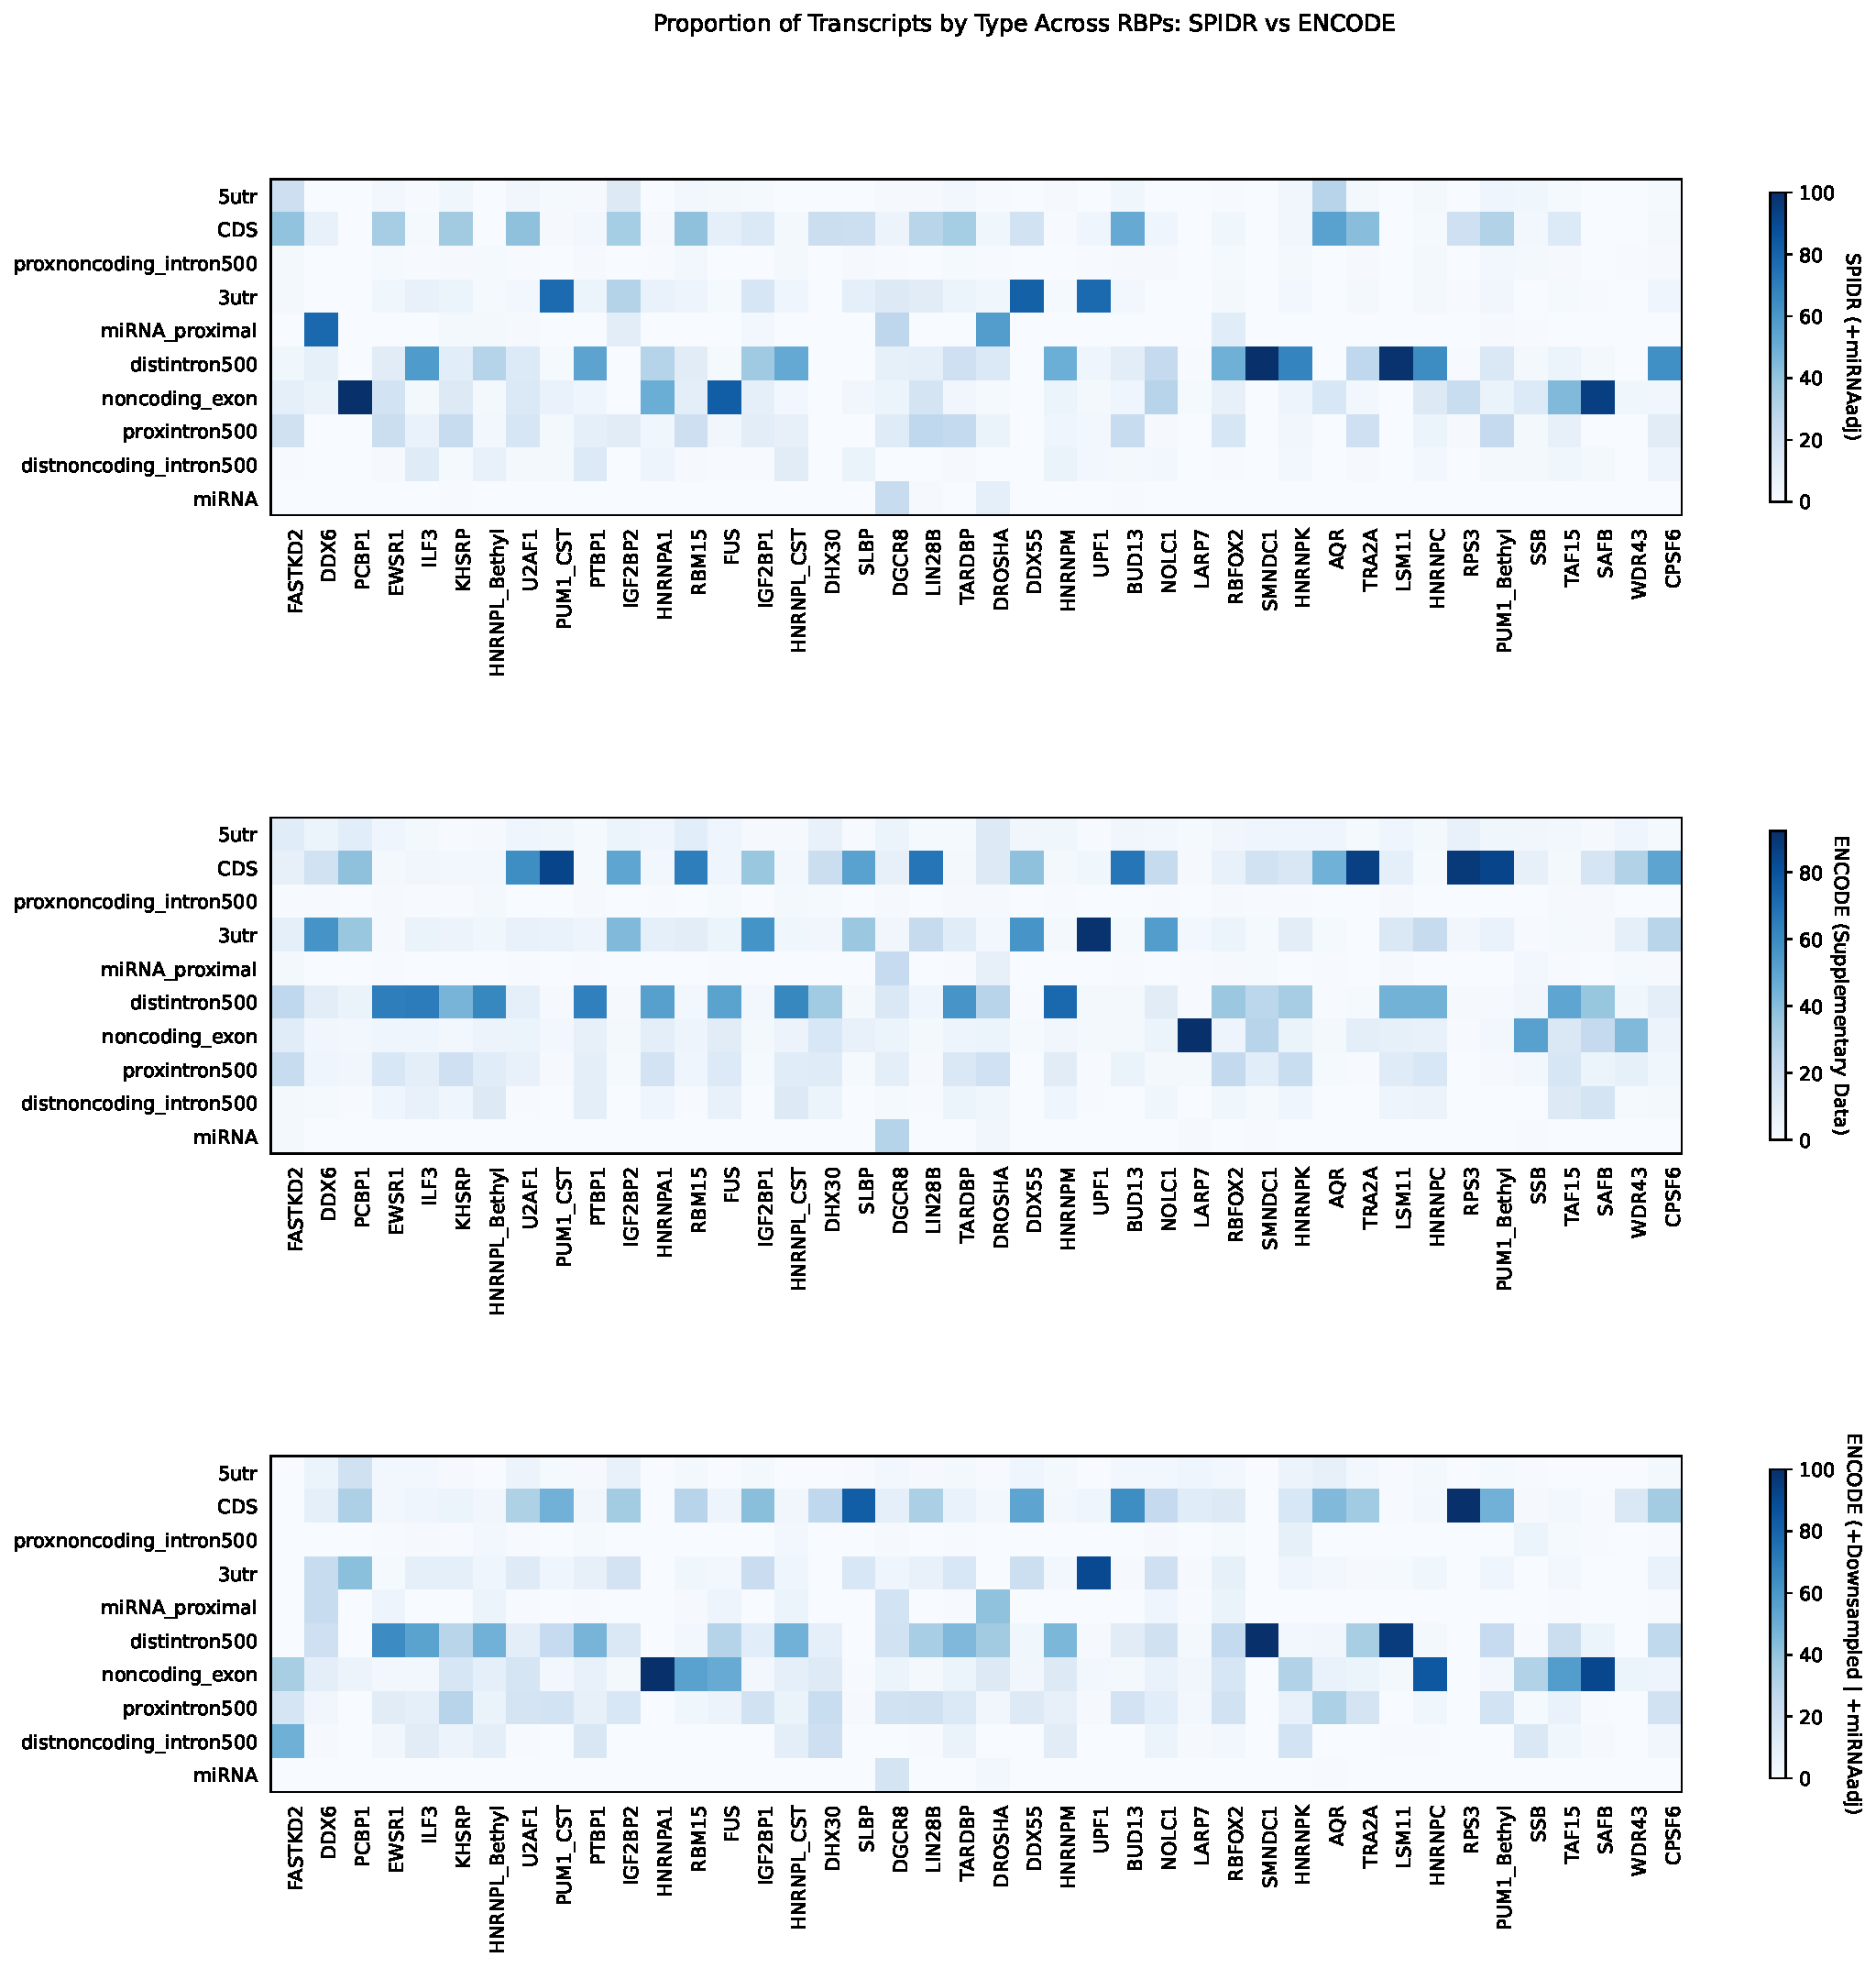
\includegraphics[scale=0.4]{../../figures/heatmap_spidr_vs_encode_miRNAadj.pdf}
        \caption[short]{Comparing ENCODE to SPIDR }
    \end{figure}
    
    \noindent We also compared the distribution of imputed transcript proportions versus the true transcript proportions. Essentially, we wanted to ensure that our observed transcript proportions were significantly different from those that we would expect by chance. Indeed, this was the case.
    \begin{figure}[ht]
        \centering
        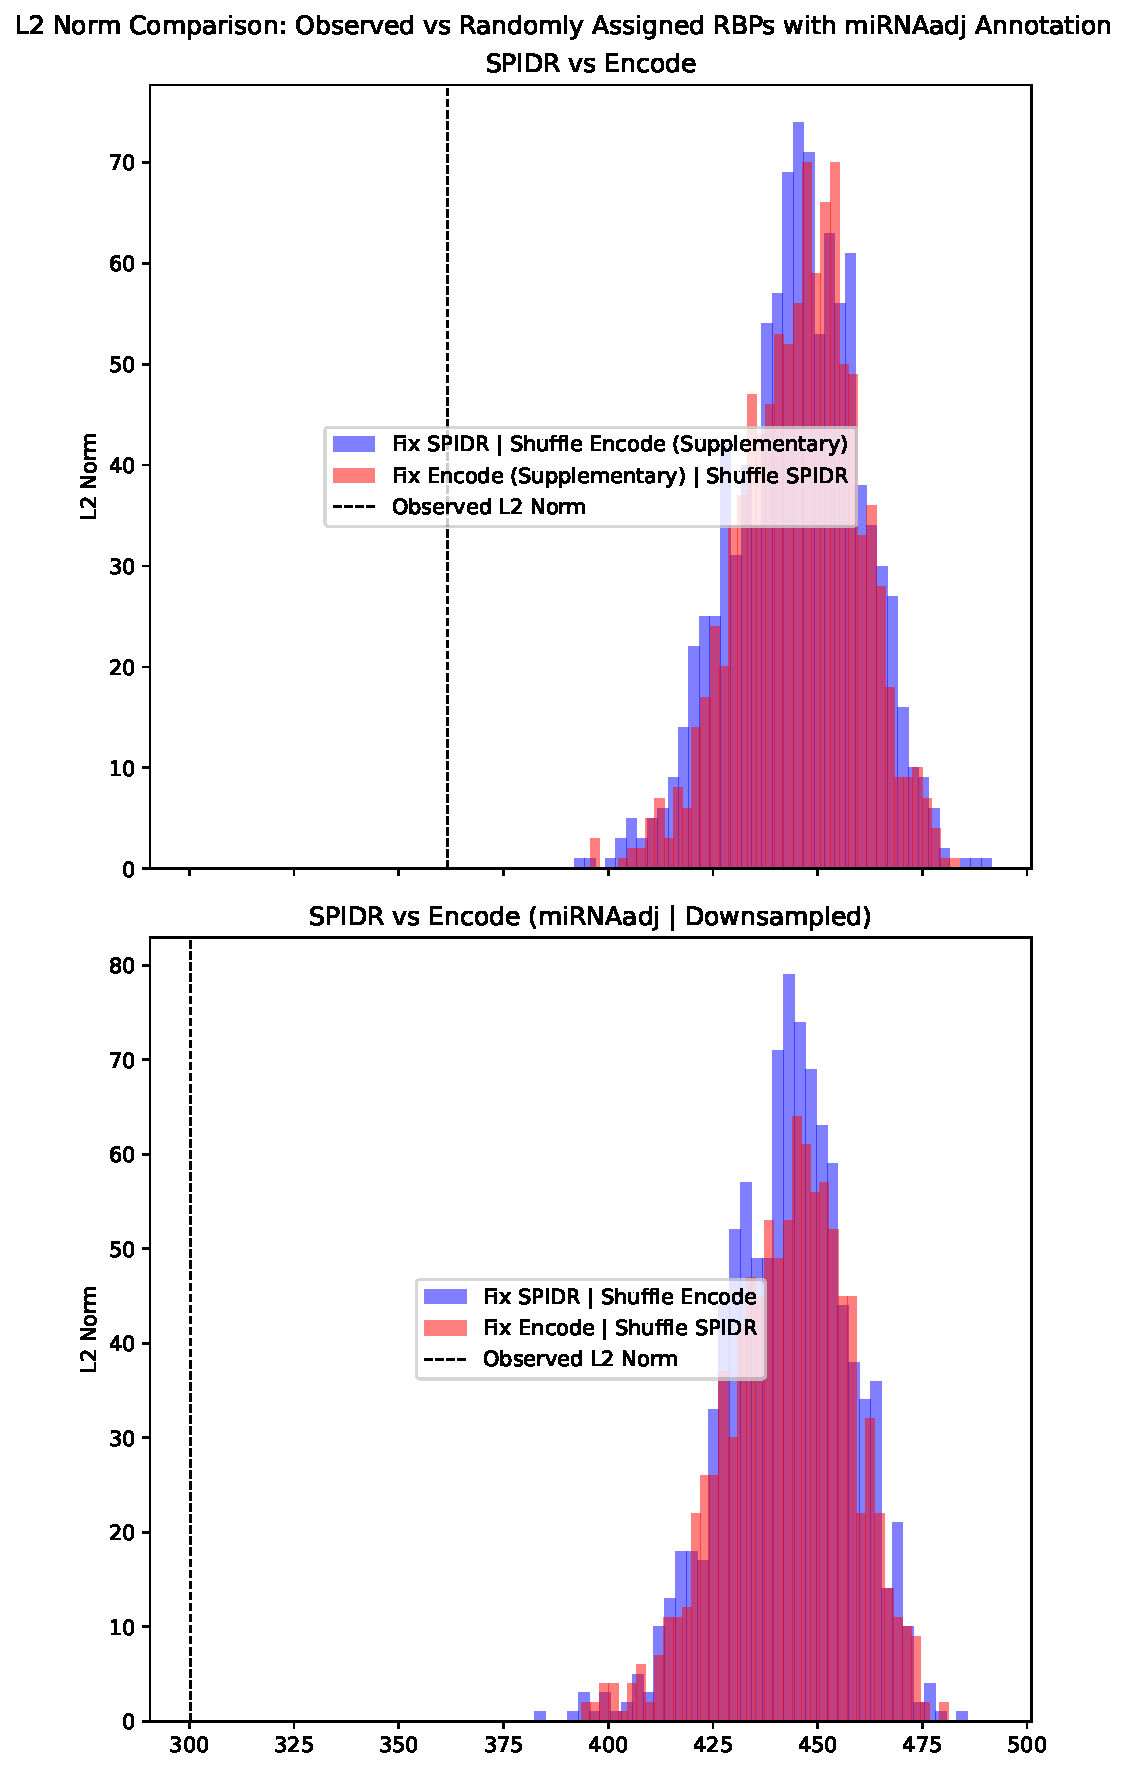
\includegraphics[scale=0.6]{../../figures/l2-shuffle-impute-with-miRNAadj.pdf}
        \caption[short]{Comparing ENCODE to SPIDR }
    \end{figure}

    \section{Glossary}
    \begin{itemize}
        \item \textbf{fastq}: A file format for storing a biological sequence and its corresponding quality scores.
        \item \textbf{bed}: A file format for storing genomic intervals. 
        \item \textbf{bedgraph}: A file format for storing genomic intervals and their corresponding values.
        \item \textbf{bowtie2}: A short read aligner.
        \item \textbf{STAR}: A short read aligner.
        \item \textbf{Snakemake}: A workflow management system.
        \item \textbf{DAG}: A data structure which tells Snakemake the dependencies between rules so Snakemake can determine how to optimally schedule rules on a system.
        \item \textbf{rule}: A step in the pipeline.
        \item \textbf{cluster.yaml}: A file that configures the \texttt{sbatch} jobs. It sets things like the account ID so jobs actually get queued, the memory per job, the number of cpus per job, the maximum time a job should run, etc.
        \item \textbf{config.yaml}: A file that configures the pipeline itself. This has parameters like the filepaths for indicies for the bowtie2 and STAR aligners.
        \item \textbf{Snakefile}: The file that actually runs the pipeline and contains all the rules. The rules are the individual steps that are run in the pipeline.
        \item \textbf{rulegraph}: A visual representation of the DAG.
        \item \textbf{mamba}: A package manager for conda packages.
        \item \textbf{conda}: A package manager for python packages.
        \item \textbf{conda-forge}: A repository of conda packages.
        \item \textbf{base environment}: The default environment that conda uses.
        \item \textbf{environment}: A collection of packages that can be used together.
        \item \textbf{environment.yml}: A file that specifies the packages that should be installed in an environment.
        \item \textbf{mambaforge}: A version of conda that uses mamba as its dependency resolver.
        \item \textbf{dependency resolver}: A tool that determines which packages need to be installed in order to satisfy the dependencies of a package.
    \end{itemize}
\end{document}